\section{INTRODUCTION}
This chapter describes the implementation of the proposed system, step by step. Since the research has been carried out by few implementation phases, those implementation phases are described as follows. 

\section{SETUP FreeRADIUS SERVER}
Ubuntu 14.04 has been taken as the host server implementation. All server implementations have been done on top of Ubuntu operating system.

\paragraph{}
\begin{center}
	\begin{figure*}[h]	
		\centering
		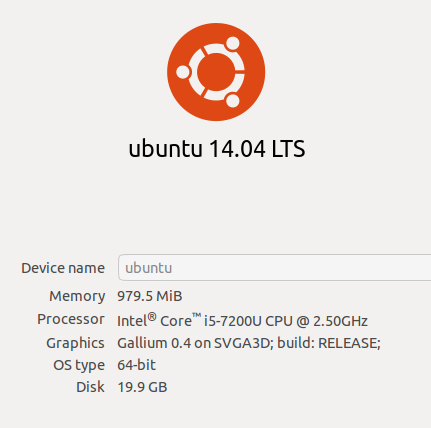
\includegraphics[width=0.4\textwidth]{ubuntu.png}
		\caption{Host server specification}
	\end{figure*}
\end{center} 

\subparagraph{NOTE : }
The host server should have root access for the implementation.

\paragraph{}
 \begin{itemize}
 	\item Install FreeRADIUS services, MySQL, PHP and other required modules\cite{freeradius}. 
 	\begin{lstlisting}
	apt-get install freeradius php-common 
	php-gd php-curl php-mail php-mail-mime 
	php-pear php-db php-mysql freeradius-mysql 
 	\end{lstlisting}
 		
 	\item Edit \verb |\etc\freeradius\clients.conf | to accept and communicate with Wi-Fi access point (IP 192.168.1.1/255.255.255.0) by adding following code snippet at the end of the file.
 	\begin{lstlisting}
 	client LBA_AP{
 	ipaddr	= 192.168.1.1
 	secret	= testing123
 	 }
 	\end{lstlisting}
 		
 		The "ipaddr" is the IP address of the Wi-Fi access point and the "secret" is the pre-shared key between RADIUS server and Wi-Fi access point. The client name is defined as \verb|"LBA_AP"|.
 		
 	\item It is known that the RADIUS protocol uses port 1812 and port 1813 for its operations. Therefore by executing following commands, allow access to the relevant ports from Ubuntu firewall.
 	\begin{lstlisting}
	ufw allow 1812
	ufw allow 1813
 	\end{lstlisting}
 		
 		
 	\item Since the technique uses MySQL database, the database has to be created and populated the tables as per the data. To create new database "lba" and create tables,
 	%\begin{appendices}
 	
 	\begin{lstlisting}
 	create database lba;

 	create table users 
 	(user_id int primarykey auto_increment,
 	user_name varchar(100) not null,
 	password varchar(100) not null,
 	allow_login int default 1);
 		
 	create table locations 
 	(id int primarykey auto_increment,
 	description varchar(45) not null,
 	AP1  varchar(45) not null,
 	AP2  varchar(45) not null,
 	AP3  varchar(45) not null,
 	AP1_name  varchar(100) not null,
 	AP2_name  varchar(100) not null,
 	AP3_name  varchar(100) not null,
 	AP1_BSSID  varchar(100) not null,
 	AP2_BSSID  varchar(100) not null,
 	AP3_BSSID  varchar(100) not null);
 		
	 create or replace view calibrated_locations as
	 select description as location,
	 min(AP1) as min_ap1,
	 max(AP1) as max_ap1,
	 min(AP2) as min_ap2,
	 max(AP2) as max_ap2,
	 min(AP3) as min_ap3,
	 max(AP3) as max_ap3 
	 from locations 
	 group by description
	 order by description asc;
 	\end{lstlisting}
 	%\end{appendices}
 		\item After creating tables, the FreeRADIUS server was configured to use the created database through PHP script. Refer authscript.php from appendix \ref{php_script}
 		
 			\subitem this PHP script handles both populating off-line training database and on-line positioning phase of the location fingerprinting technique. The following code snippet directs RADIUS server to execute PHP script.\cite{freeradius_2}
 			
 			Edited \verb|/etc/freeradius/sites-enabled/default| file and added the code at the end of the block \verb|authorize {}|\cite{freeradius_php}
 			
 		\begin{lstlisting}
 		update control {
 		Auth-Type := `/usr/bin/php -f
 		/etc/freeradius/authscript.php 
 		'%{User-Name}' 
 		'%{User-Password}' 
 		'%{Client-IP-Address}'`
 			}
 		\end{lstlisting} 
 	
 		\subitem Now FreeRADIUS server is ready and restarted by using following commands.
 		\begin{lstlisting}
 		/etc/init.d/freeradius stop
 		/etc/init.d/freeradius start
 		\end{lstlisting}
 \end{itemize}

\newpage
\section{SETUP WI-FI ROUTER}
The Wi-Fi router has been configured to forward all authentication requests to the FreeRADIUS server. The used Wi-Fi router is DCP LINK ,model "DCP-WR300N".

%\paragraph{}
\begin{center}
	\begin{figure*}[h]	
		\centering
		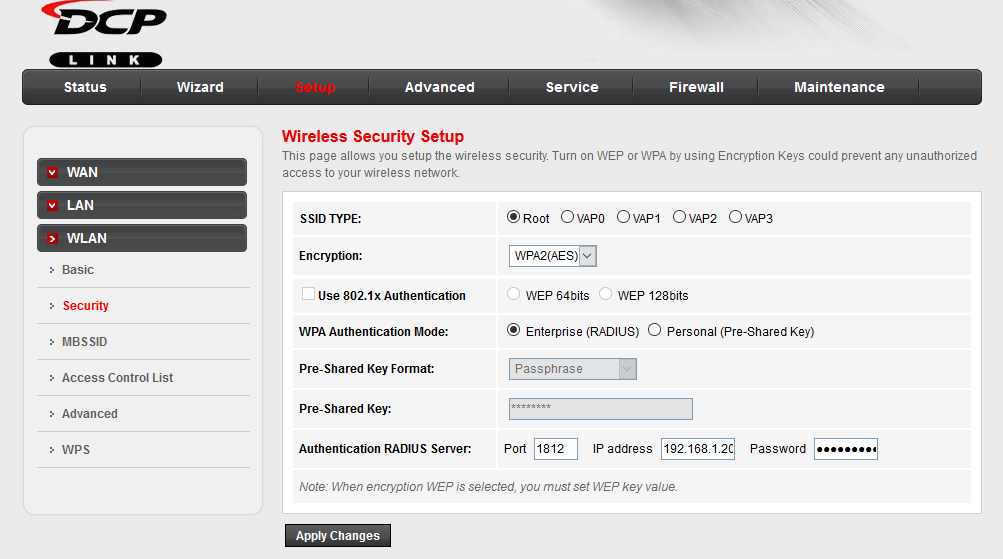
\includegraphics[width=1\textwidth]{router_config.png}
		\caption{Wi-Fi router configuration}
	\end{figure*}
\end{center} 

Router configured for WPA2(AES) encryption and WPA Authentication mode set to Enterprise(RADIUS). Authentication RADIUS server port has configured as 1812, IP address as 192.168.1.20/255.255.255.0 and the most important pre-shared secret is set as per the FreeRADIUS server's \verb|\etc\freeradius\clients.conf| file. It is pretty straight forward and easy to configure Wi-Fi router to authenticate via FreeRADIUS server. FreeRADIUS server and W-Fi router are connected by using wired connection.

\section{DEVELOP ANDROID MOBILE APPLICATION}
The Android mobile application is the tool that used to collect Wi-Fi signal strength of each location with respect to each access point. User has to nominate three(03) access  points from available access points list which are provided in the application settings menu, by scanning Wi-Fi access points in real time, for the authentication process.

\begin{center}
	\begin{figure*}[h]	
		\centering
		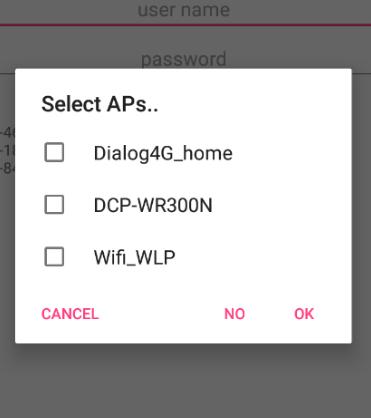
\includegraphics[width=0.5\textwidth]{select_ap.png}
		\caption{Select Access Points first}
	\end{figure*}
\end{center}

\newpage
This selected three(03) access points information will be collected by the application and make a JSON object to send to the authentication server. Sample JSON object is as follows.\cite{jsonlint}
	\begin{lstlisting}
	{
		"name": "username",
		"password": "userpassword",
		"ap3name": "AP3_name",
		"ap3": -69,
		"ap3_BSSID": "c8:b5:ad:8b:dd:a0",
		"ap2name": "AP2_name",
		"ap2": -72,
		"ap2_BSSID": "08:5b:0e:10:2b:0a",
		"ap1name": "AP1_name",
		"ap1": -79,
		"ap1_BSSID": "2a:5b:0e:0f:e6:aa",
		"desc": "",
		"save": "n"
	}
	
	\end{lstlisting}

\newpage
Method wpa2enterprise() stands for providing necessary information to the FreeRADIUS server to authenticate user. \cite{wifi_connect}
Refer appendix \ref{android_api} for wpa2enterprise() method.

\begin{center}
	\begin{figure*}[h]	
		\centering
		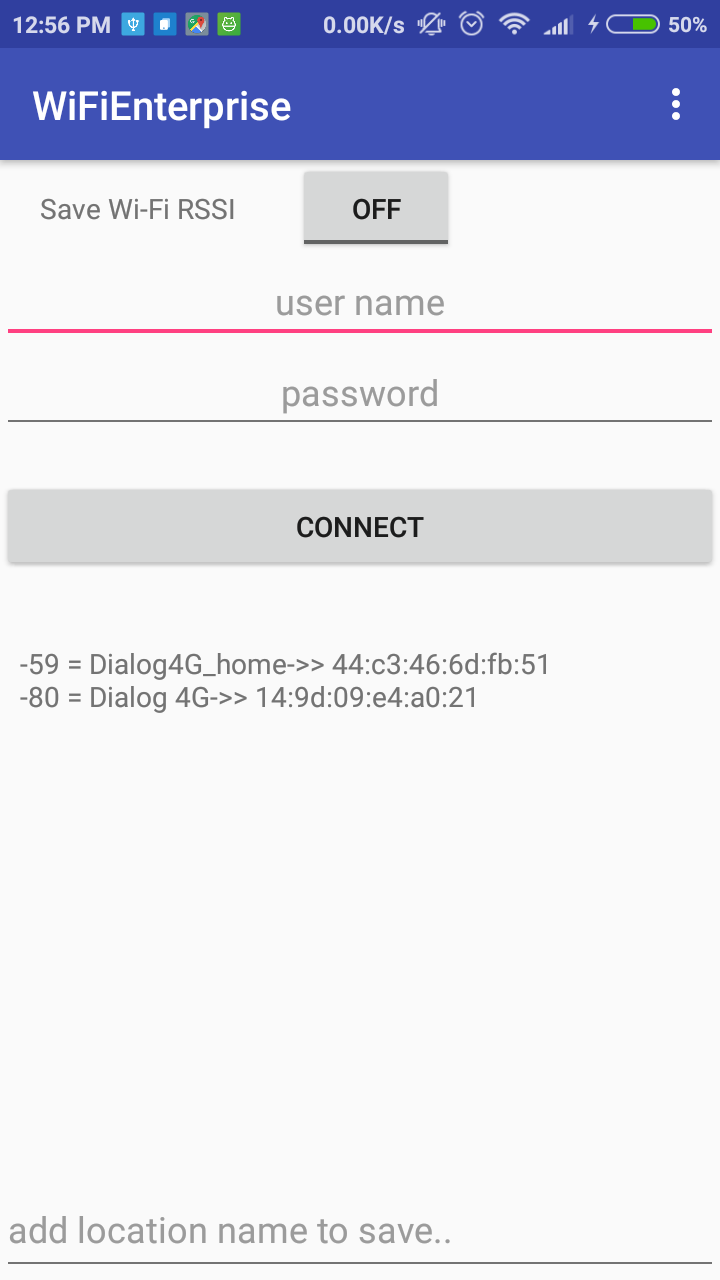
\includegraphics[width=0.4\textwidth]{mobile_app.png}
		\caption{Android Mobile Application}
	\end{figure*}
\end{center}

\newpage
\section{DEVELOP BACK END ADMINISTRATION PANEL}
Back end administration panel is web based back end application which supports to the administrator to control Wi-Fi users such as add new user, allow and deny access to the existing users.  

\begin{center}
	\begin{figure*}[h]	
		\centering
		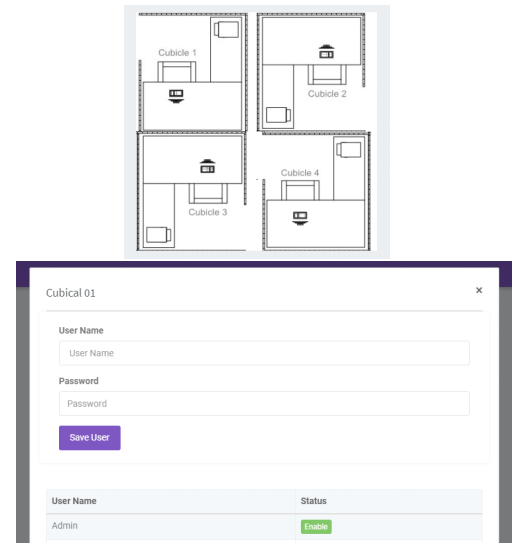
\includegraphics[width=0.6\textwidth]{backend.png}
		\caption{Back end admin panel}
	\end{figure*}
\end{center}

\newpage
\section{FREERADIUS STATIC TESTING TOOL}
NTRPing is a useful tool for testing installation of the RADIUS server. By using this tool, it is possible to simulate authentication and accounting requests and send them to the RADIUS server. 

\begin{center}
	\begin{figure*}[h]	
		\centering
		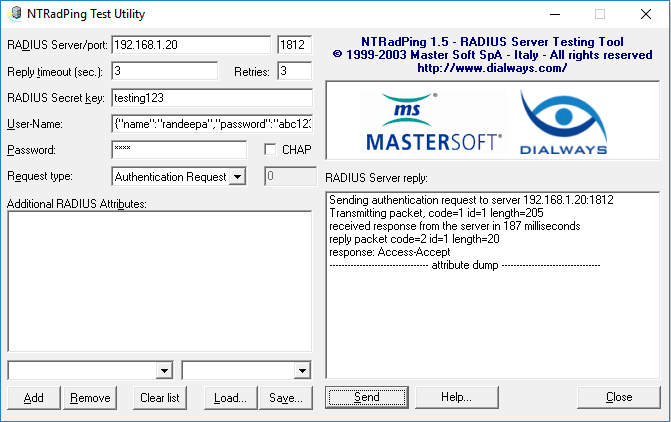
\includegraphics[width=0.8\textwidth]{ntrping.png}
		\caption{NTRPing tool}
	\end{figure*}
\end{center}

It is easy to check the RADIUS server by using this tool since NTRPing tool is acting like NAS client.\cite{ntrping_tool}

%\section{LOCATION FINGERPRINT DATA}